\documentclass[
  style=pd,
  %blackslide,
  %mode=handout,
  %mode=print,
  clock
]{powerdot}

\pdsetup{
  lf={Small Tutorial on the Usage of my RIKEN GEANT4 ...},  % left footer
  rf={RIBF 3$^{\text{rd}}$ floor TV-room, January 9$^{\text{th}}$, 2009}, % right footer
  theslide=\arabic{slide},
  logohook=c,
  logopos={.06\slidewidth,.95\slideheight},
  logocmd={\includegraphics[width=.09\slidewidth]{/home/doornen/Presentations/template/nc-logo-light-grey_no-text.eps}}
}


%
% packages
\usepackage{graphicx}
\usepackage{amssymb}
\usepackage{amsmath}

\usepackage[10pt]{type1ec}          % use only 10pt fonts
\usepackage[T1]{fontenc}
\usepackage{CJKutf8}
\usepackage[german, USenglish]{babel}
\usepackage{xspace}
\usepackage[overlap, CJK]{ruby}
\renewcommand{\rubysep}{-0.2ex}

% 
% some easy commands
\newcommand{\ts}{\textsuperscript}
\newcommand{\er}{\rule{0pt}{0pt}}  % empty rule
\newcommand{\ur}{\rule{1pt}{1pt}}  % unit rule
\newcommand{\gr}[1][0,0]{\psgrid[gridwidth=.015,gridcolor=red,subgridwidth=.005,subgridcolor=red,gridlabelcolor=red](#1)(-13,-9)(13,9)}
\newcommand{\etal}{\textit{et al.}}
\newcommand{\psbar}[1][.55]{\er\rput(#1ex,1.1ex){\rule{.7ex}{0.05ex}}}
\newcommand{\lambdabar}{\ensuremath{\psbar\lambda}}
\newcommand{\power}[1]{$\times 10^{#1}$}
\newcommand{\beupl}{\ensuremath{B(E2;~0^+_{\mathrm{g.s.}}\rightarrow2^+_1)}\xspace} % long B(E2)
%$B(E2$; $0^{+}_{g.s.} \rightarrow 2^{+}_{1}$)
\newcommand{\beup}{\ensuremath{{B( E2)\!\!\uparrow}}\xspace}  % short B(E2)


%% For testing text height.
\makeatletter
\def\slidearea{\psframe[linecolor=blue](\slidewidth,\slideheight)}
\def\textarea{\psframe[linecolor=red](\pd@@textwidth,-\pd@@textheight)}
\def\textheightrule{\rput[tl](0,0){\red\rule{1pt}{\pd@@textheight}}}
\def\textwidthrule{\rput[tl](0,0){\red\rule{\pd@@textwidth}{1pt}}}
\makeatother

%%%%%%%%%%%%%%%%%%%%%%%%%%%%%%%%%%%%%%%%%%%%%%%%%
\begin{document}
\begin{CJK}{UTF8}{min}
  
  %%-----------------------------------------------
  \author{Pieter Doornenbal\\[10mm]\includegraphics[width=7cm]{/home/doornen/Presentations/template/nc-logo-color.eps}\\[1cm]}
  \date{\small }
  \title{Small Tutorial on the Usage of my RIKEN GEANT4 Package}

%%-----------------------------------------------
  \begin{displaytestslide}[logopos=,toc=]{}
  \rput(0,0){\includegraphics[width=10cm]{/home/doornen/Presentations/template/nc-logo-color.eps}}
\end{displaytestslide}


%%-----------------------------------------------
\maketitle[logopos=]


%%-----------------------------------------------

%oooooooooooooooooooooooooooooooooooooooooooooooo
\begin{slide}[toc=]{Outline}{
    \tableofcontents[]
  }
\end{slide}

%%-----------------------------------------------
\section[toc=Introduction]{Introduction}

%oooooooooooooooooooooooooooooooooooooooooooooooo
\begin{slide}{Introductive Remarks}
  \begin{itemize}\itemsep 15pt
  \item The Simulation package is intended to simulate the $\gamma$-ray detection response for different arrays employed presently
    or in the future at the RIBF.
  \item Why are simulations necessary?
    \begin{itemize}\itemsep 10pt { \small
      \item Intensity and energy resolution estimations prior to an experiment
      \item Optimize the geometry for present and future arrays
      \item Understand lineshapes of observed spectra (lifetime, doublets, Compton-scattering, escape peaks, etc.)
      \item Intensity determinations for observed peaks in in-beam experiments
      }
    \end{itemize}
  \end{itemize}
\end{slide}

%oooooooooooooooooooooooooooooooooooooooooooooooo
\begin{slide}[toc=]{Installation Requirements}
  \begin{itemize}\itemsep 15 pt
  \item ROOT, preferably the newest version
  \item GEANT4 (version>=g4.9.0.p01)
  \item CLHEP (Class Library with High Energy Physics)
  \item DAWN (Drawer for Academic WritiNgs)
  \item  Visit \newline \newline  
    {\ttfamily http://geant4.slac.stanford.edu/installation/} \newline \newline 
    for an installation guide.
  \end{itemize}
\end{slide}

%oooooooooooooooooooooooooooooooooooooooooooooooo
\begin{slide}{Installing the Simulation Package}
\begin{itemize}\itemsep13pt
\item Copy {\ttfamily Geant4Riken.0.5.7.tar.gz} from \newline
  {\ttfamily /rarf/u/pieter/} \newline
  (Starting from next week)
\item Unpack the file with: \newline
  {\ttfamily tar -zxf Geant4Riken.0.5.7.tar.gz}\pause
\item Five subdirectories will be created, namely:\newline
  {\ttfamily EventGenerator\newline
    EventBuilderRIKEN\newline
    Reconstructor\newline
    tutorial} (Empty dummy folder) \newline
  {\ttfamily manual} (Not finished, also these transparancies.)
\end{itemize}
\end{slide}

%oooooooooooooooooooooooooooooooooooooooooooooooo
\begin{slide}{The Three Simulations Steps}
  The simulation is divided into three steps because they are basically independent of each other. \linebreak
  \begin{itemize}\itemsep10pt
  \item The Event Generator
    \begin{itemize} { \small
      \item $\gamma$-ray distribution and Doppler shift
      \item Energy loss in the target
      \item Velocity shift after fragmentation (Borrel \etal)
        %\begin{equation}
        %  \frac{v_{f}}{v_{p}} = \sqrt{1-\frac{B_{n}(A_{P}-A_{F})}{A_{P}E_{F}}}
        %\end{equation}
      \item Parallel momentum distribution (Goldhaber \etal)
        %  \begin{equation}
        %    \sigma_{||}=\sigma_{0}^{2} \frac{A_{F}(A_{P}-A_{F})}{A_{P}-1}
        %  \end{equation}
      }
    \end{itemize}
  \item The Event Builder
    \begin{itemize} { \small
      \item Inserting the detector geometry, target holder, beam pipe, etc.
      \item $\gamma$-ray interaction with the material
      }
    \end{itemize}
  \item The Reconstructor
    \begin{itemize} { \small
      \item Doppler shift correction
      \item $\gamma$-ray fold, energy resolution, lineshape, efficiency, etc.
      }
    \end{itemize}
  \end{itemize}
\end{slide}

%oooooooooooooooooooooooooooooooooooooooooooooooo
\begin{slide}[toc=]{The Simulation Procedure}
  \rput[tl](0,0){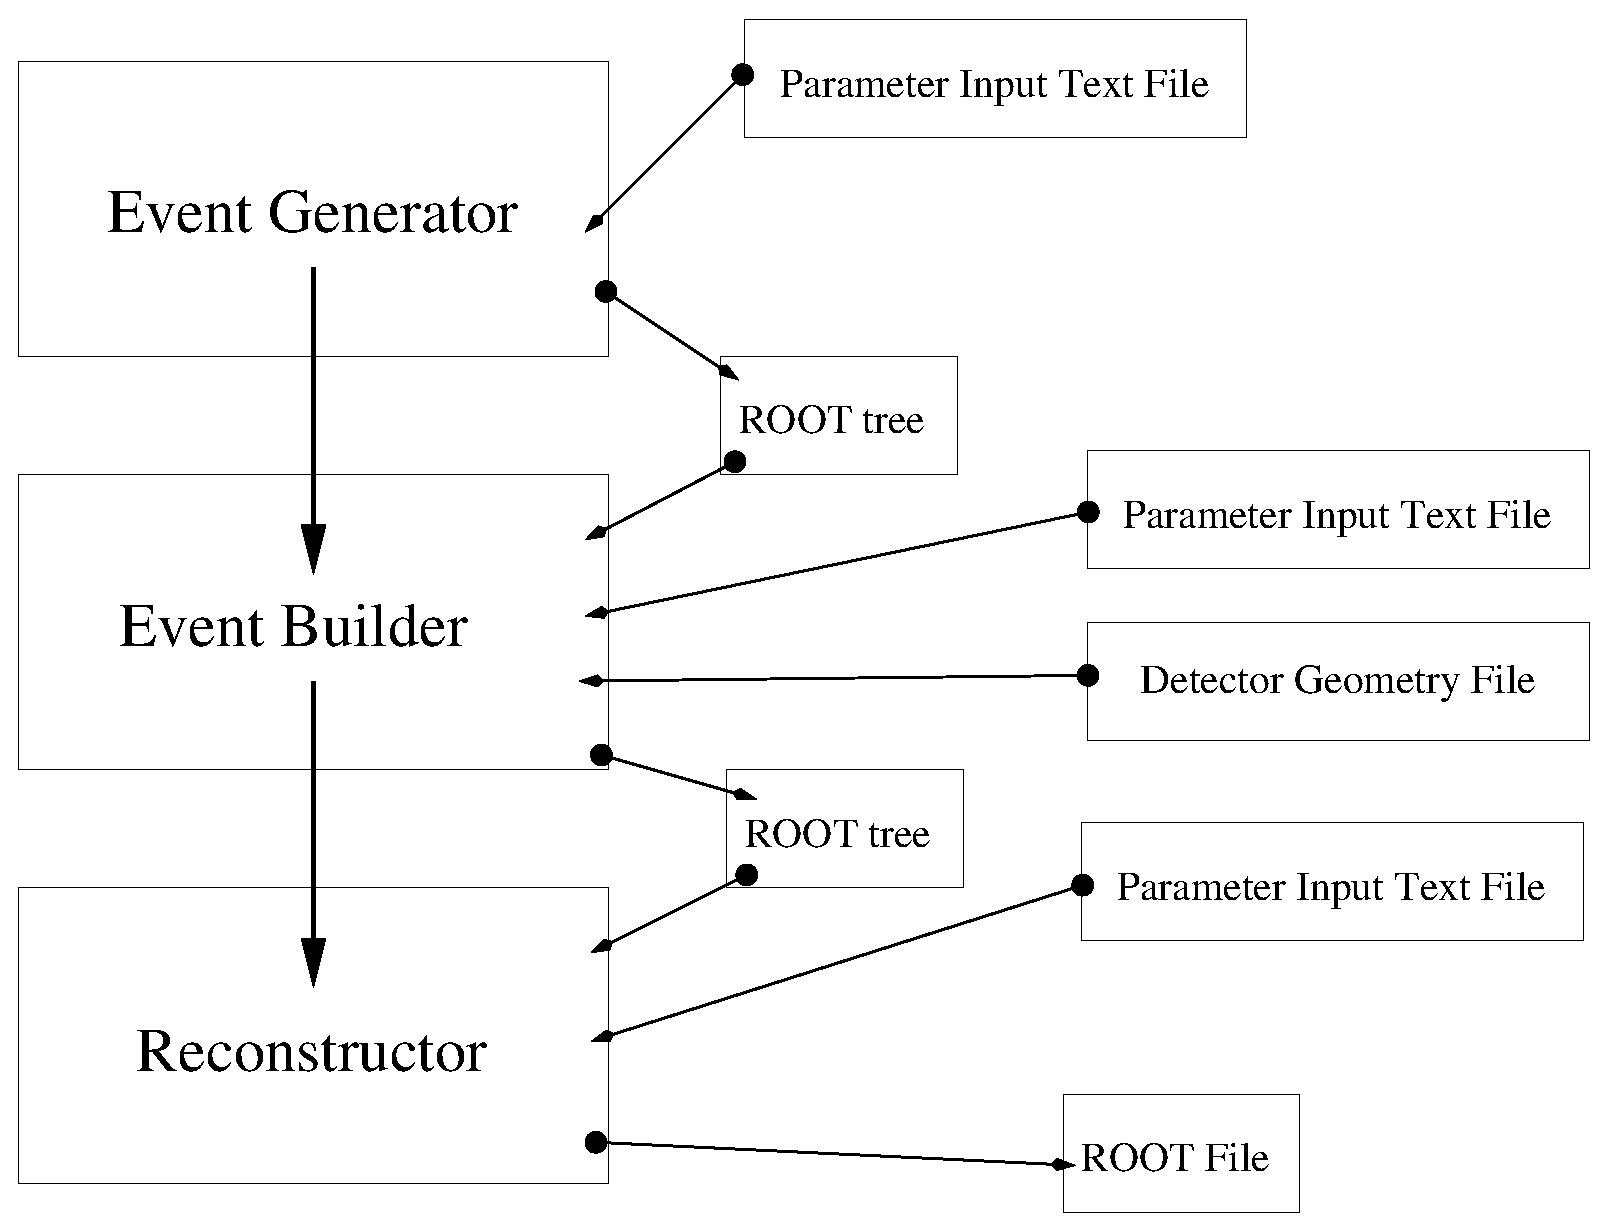
\includegraphics[width=10cm]{./SimulationScheme.eps}}
\end{slide}

%%-----------------------------------------------
\section[]{The Event Generator}

%oooooooooooooooooooooooooooooooooooooooooooooooo
\begin{slide}{The Input File}
  \begin{itemize}\itemsep 15pt
  \item The Input File can be found under {\ttfamily ./input/EventGenerator.in}
  \item Only the most important input keywords are listed. The manual, still under construction,
    will cover all.
    \begin{itemize} { \small \ttfamily
        \item BEAMISOTOPE $A_{P}$ $Z_{P}$ $Q_{P}$
        \item BEAMENERGY $E_{P}$ $\Delta E(FWHM)_{P}$
        \item BEAMPOSITION $X$ $FWHM_{X}$ $Y$ $FWHM_{Y}$
        \item TARGET $Type$ $Size_{X}$ $Size_{Y}$ $Thickness_{Z}$ 
        \item MASSCHANGE $\Delta A$ $\Delta Z$
        \item GAMMAINPUT $File_{\gamma-in}$
        \item NUMBEROFEVENTS $N_{events}$
        \item OUTPUFILENAME $File_{out}$
        \item DEDXTABLE Option$_{dEdX}$ $File_{P}$ $File_{E}$
        \item END
      }
    \end{itemize}
  \end{itemize}
\end{slide}

%oooooooooooooooooooooooooooooooooooooooooooooooo
\begin{slide}{The Gamma Input File}
  \rput[tl](1,.5){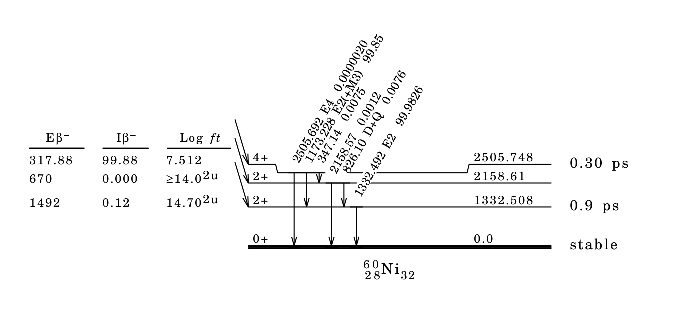
\includegraphics[width=9cm]{./60CoBetaDecay.eps}}\pause
  \rput[tl](1.,-3.5) {
    \small
    \parbox{8.0cm} {\ttfamily
      LEVEL  0  00.00 0000.000 0.00\linebreak
      LEVEL  1  00.12 1332.510 0.90\linebreak
      LEVEL  2  00.00 2158.610 0.00\linebreak
      LEVEL  3  99.88 2505.748 0.30\linebreak
      DECAY  1  0 99.9826\linebreak
      DECAY  2  1 00.0076\linebreak
      DECAY  2  0 00.0012\linebreak
      DECAY  3  2 00.0075\linebreak
      DECAY  3  1 99.85\linebreak
      DECAY  2  0 00.0000020\linebreak
    }
  }\pause
       {\color{red} No $\gamma$-$\gamma$ angular correlations!}
\end{slide}

%oooooooooooooooooooooooooooooooooooooooooooooooo
\begin{slide}{Using dEdX Tables}
  Instead of letting GEANT4 calculate the energy loss in the target, 
  dEdX tables can be used. For thick targets, this will speed
  up the simulation process. The input table has the following form:\linebreak
  \rput[tl](1.,0.){
    \small
    \parbox{8.0cm} {\ttfamily
      dEdX  267.5 0.336315 \linebreak
      dEdX  265.0 0.338156 \linebreak
      . \linebreak
      . \linebreak
      . \linebreak
      END 
    }
  }
  \rput[tl](0.,-3.){
    \parbox{11.0cm} {
      \begin{itemize}\itemsep 6pt
      \item Up to 50 values can be inserted.
      \item Energy loss is given in MeV/(mg/cm$^{2}$).
      \item The First two point define the energy spacing for a linear interpolation.
      \item Use for example the goodies section in LISE++ (based on ATIMA1.2)
      \end{itemize}
    }
}
\end{slide}

%%-----------------------------------------------
\section[]{The Event Builder}

%oooooooooooooooooooooooooooooooooooooooooooooooo
\begin{slide}{The Input File}
  \begin{itemize}\itemsep 15pt
  \item The Input File can be found under {\ttfamily ./input/EventBuilder.in}
  \item Only the most important input keywords are listed. The manual, still under construction,
    will cover all.
    \begin{itemize} { \small {\ttfamily
        \item INPUFILENAME $File_{in}$
        \item OUTPUFILENAME $File_{out}$
        \item DALI2INCLUDE $Option_{DALI2}$
        \item DALI2ENERGYRESOLUTION $i$ $a$ $b$\linebreak
        }If $i=1$:  $\Delta E (FWHM) = a + bx$ keV. \linebreak
        If $i=2$: $\Delta E (FWHM) = ax^{b}$ keV.
        {\ttfamily
        \item BETARESOLUTION $a$\linebreak
          $a=\Delta \beta / \beta (FWHM)$
         \item TARGETHOLDERINCLUDE $Option_{TargetHolder}$
         \item BEAMPIPEINCLUDE $Option_{BeamPipe}$
         \item DALI2FIINCLUDE $Option_{FI}$
         \item END
        }
      }
    \end{itemize}
  \end{itemize}
\end{slide}

%oooooooooooooooooooooooooooooooooooooooooooooooo
\begin{slide}{The DALI2 Geometry Input File}
  \begin{itemize}\itemsep 10pt
  \item The Input File can be found under: {\ttfamily ./geometry/dali2\_geometry\_in.txt}
  \item It has the following structure:\linebreak
    {\ttfamily POSX POSY POSZ PSI THETA PHI ROTSIGN DETTYPE\linebreak
      .\linebreak
      .
    }
  \item Up to 182 detectors (check the global variable defined in {\ttfamily Globals.hh})
  \item Three different NaI detector types can be chosen:
    \begin{itemize} { \small
      \item {\ttfamily DETTYPE = 0} Saint-Gobain 
      \item {\ttfamily DETTYPE = 1} Scionix  
      \item {\ttfamily DETTYPE = 2} DALI1 
      }
    \end{itemize}
  \item The crystals are not centered with respect to their housing
  \item {Take a look at {\ttfamily \color{red} \bf  ./src/Dali2.cc} 
    and {\ttfamily \color{red} \bf./include/Dali2.hh} !}
  \end{itemize}
\end{slide}

%%-----------------------------------------------
\section[]{The Reconstructor}

%oooooooooooooooooooooooooooooooooooooooooooooooo
\begin{slide}{The Input File}
  \begin{itemize}
  \item The Input File can be found under: {\ttfamily ./Dali2Reconstructor.in}\linebreak
    \begin{itemize}\itemsep 3pt { \small 
        \item {\ttfamily INPUFILENAME} $File_{in}$
        \item {\ttfamily OUTPUFILENAME} $File_{out}$
          %\item DALI2INCLUDE $Option_{DALI2}$
        \item {\ttfamily FIFIND} $i$
          \linebreak
          If $i=1$, the average first interaction point of a full 
          energy peak $\gamma$-ray (with fold=1) is determined for every crystal. 
        \item {\ttfamily BETADOPPLERAVERAGE} $a$\linebreak 
          The average $\beta$-value used for the Doppler correction.
        \item {\ttfamily BETATOFAVERAGE} $a$ \linebreak
          The average $\beta$-value in front of the target. This value is necessary for an event-by-event
          Doppler correction with different incoming velocities.
        \item {\ttfamily DECAYPOSITION} $z$ %\linebreak
          %The average $z$-positon along the beam-axis shifts as a function of the excited states' lifetimes. This
          %value can be inserted to correct for this effect.
        \item {\ttfamily STATISTICSREDUCTIONFACTOR} $a$ %\linebreak
          %If you have simulated many events in the second step and 
          %want to see how the Doppler corrected response might
          %have looked like for limited statistics you can reduce your statistics by putting a value $a\gt1$.
        \item {\ttfamily END} 
      }
    \end{itemize}
  \end{itemize}
\end{slide}
%%-----------------------------------------------
\section[]{Simulation Examples}

%oooooooooooooooooooooooooooooooooooooooooooooooo
\begin{slide}{DALI2 Efficiency with $^{60}$Co Source}
  \begin{itemize} 
    \item Structure of the Event Generator Input File:\linebreak 
      {\ttfamily \small
        GAMMAINPUT ./input/60Co.in\linebreak
        NUMBEROFEVENTS 100000\linebreak
        OUTPUTFILE ../tutorial/60CoGenerator.root\linebreak
        END
      }
    \item Structure of the Event Builder Input File:\linebreak
      {\ttfamily \small
        INPUTFILE ../tutorial/60CoGenerator.root\linebreak
        OUTPUTFILE ../tutorial/60CoBuilder.root\linebreak
        DALI2INCLUDE 1\linebreak
        DALI2ENERGYRESOLUTION 2 2.2795 0.5\linebreak
        END
      }
    \item Structure of the Reconstructor Input File:\linebreak
      {\ttfamily \small
        INPUTFILE ../tutorial/60CoBuilder.root\linebreak
        OUTPUTFILE ../tutorial/60CoReconstructor.root\linebreak
        SPECTRABINANDRANGE 400 0. 4000.\linebreak
        END
      }
  \end{itemize}
\end{slide}


%oooooooooooooooooooooooooooooooooooooooooooooooo
\begin{slide}[toc=,bm=]{DALI2 Efficiency with $^{60}$Co Source}
  \begin{itemize}
\item Set the environment from my {\ttfamily .bashrc} or by typing {\ttfamily sh setup.sh}
  \item Run the Event Generator in the directory {\ttfamily EventGenerator} with:\linebreak
    {\ttfamily  EventGenerator run\_nothing.mac} 
  \item Run the Event Builder in the directory {\ttfamily EventBuilderRIKEN} with:\linebreak
    {\ttfamily  EventBuilder run\_nothing.mac} \linebreak
    Omitting {\ttfamily run\_nothing.mac} will bring you into the interactive mode, from which you 
    can take a look of the geometry by typing:\linebreak
    {\ttfamily /vis/viewer/flush}
  \item Open a ROOT session in the directory {\ttfamily Reconstructor} and 
    build the shared library using ACLIC by typing:\linebreak
    {\ttfamily root[].L Dali2Reconstructor.C+}\linebreak
    and run the script with \linebreak
    {\ttfamily root[]Dali2Reconstructor()}
  \end{itemize}
\end{slide}

%oooooooooooooooooooooooooooooooooooooooooooooooo
\begin{slide}{The First Excited State in $^{36}$Ca from the 1n-Knockout Reaction}
\begin{itemize}
\item Structure of the Event Generator Input File:\linebreak 
  {\ttfamily \small
    BEAMISOTOPE 37 20 20\linebreak
    BEAMENERGY 195.7 6.06\linebreak
    BEAMPOSITION 0.0 1.0 0.0 1.0\linebreak
    BEAMANGLE 0.0 0.65 0.0 360.0\linebreak
    TARGET 2 7.0 7.0 700\linebreak
    TARGETANGULARBROADENING 1 0.6\linebreak
    MASSCHANGE 1 0\linebreak
    BORREL 1 8.\linebreak
    GOLDHABER 1 90.\linebreak
    GAMMAINPUT ./input/36ca.in\linebreak
    NUMBEROFEVENTS 50000\linebreak
    DEFAULTCUTVALUE 0.001\linebreak
    OUTPUTFILE ../tutorial/36CaGenerator.root\linebreak
    DEDXTABLE 1 ./dEdXTables/CaOnBe.in ./dEdXTables/CaOnBe.in\linebreak
  }
\end{itemize}


\end{slide}

%oooooooooooooooooooooooooooooooooooooooooooooooo
\begin{slide}[toc=,bm=]{The First Excited State in $^{36}$Ca from the 1n-Knockout Reaction}
\begin{itemize}
\item Structure of the Event Builder Input File:\linebreak 
  {\ttfamily \scriptsize
    INPUTFILE ../tutorial/36CaGenerator.root\linebreak
    OUTPUTFILE ../tutorial/36CaBuilder.root\linebreak
    DALI2INCLUDE 1\linebreak
    %DALI2FIINCLUDE 1\linebreak
    DALI2ENERGYRESOLUTION 2 2.2795 0.5\linebreak
    POSDETECTORONTARGETRESOLUTION .3\linebreak
    POSDETECTORAFTERTARGETDISTANCE 100.\linebreak
    POSDETECTORAFTERTARGETRESOLUTION .3\linebreak
    BETARESOLUTION 0.001\linebreak
    END
  }
\item Structure of the Reconstructor Input File:\linebreak
  {\ttfamily \small  \scriptsize
    INPUTFILE ../tutorial/36CaBuilder.root\linebreak
    OUTPUTFILE ../tutorial/36CaReconstructor.root\linebreak
    SPECTRABINANDRANGE 400 0. 8000.\linebreak
    BETADOPPLERAVERAGE 0.5459\linebreak
    BETATOFAVERAGE 0.5631\linebreak
    DECAYPOSITIONZ 0.0\linebreak
    END
  }
\end{itemize}
\end{slide}


%%-----------------------------------------------
\section[toc=,bm=---]{THE END}

%__________________________________________________________________________________________________
%__________________________________________________________________________________________________
%__________________________________________________________________________________________________

%oooooooooooooooooooooooooooooooooooooooooooooooo
\begin{slide}[toc=,bm=]{}
  \begin{center}
    {\bf \textit{\Huge Backup slides from now}}
  \end{center}
\end{slide}

\end{CJK}
\end{document}
